\chapter{Arguing Affirmative Action}

In this lecture we take up affirmative action as a new test of an older question. The background claim, carried forward from the Rawls discussion, is that justice may not be a matter of rewarding virtue or moral desert. Sandel now moves that issue from income and wealth to opportunities, admissions, and hiring. The chapter therefore unfolds in two stages: first, we sort through the competing arguments for and against affirmative action in the Hopwood case; then, having pressed those arguments to their limit, we turn to Aristotle and the teleological idea that justice depends on the purpose of the practice itself.

\section{From Rawls to Hopwood}

The opening distinction is schematic but decisive. Rawls had argued that distributive justice should not be understood as the direct reward of moral worth. Sandel recalls that point in order to ask whether admission to a university, or access to opportunity more generally, can be treated as something we deserve in the strong moral sense.

\begin{equation}
\text{moral desert} \neq \text{legitimate expectations}
\end{equation}

\begin{equation}
\text{distributive justice}
\Longrightarrow
\text{opportunities, hiring decisions, admission standards}
\end{equation}

The case used to reopen the issue is Cheryl Hopwood's application to the University of Texas Law School. Sandel gives the details in a deliberately concrete order: Hopwood worked her way through school, earned a strong academic record, took the admissions test, and applied to a law school that was then using race and ethnicity as admissions factors. The point of the narrative is not biography for its own sake. It is to make the later fairness question feel earned.

Two numerical facts matter in the presentation of the case. First, Hopwood's grade point average is part of what gives her complaint force. Second, the university's own rationale depends on a demographic claim about the state it serves.

\begin{align}
\text{Hopwood GPA} &\approx 3.8,\\
\text{Texas African-American + Mexican-American share} &\approx 40\%.
\end{align}

Sandel also introduces the admissions comparison that animates Hopwood's complaint. The transcript does not provide a formal admissions formula, so we keep the notation deliberately schematic.

\begin{equation}
\text{academic index} \sim (\text{grades},\ \text{test scores})
\end{equation}

\begin{equation}
\text{lower academic index admitted}
\qquad
\text{while Hopwood rejected}
\end{equation}

At this stage the lecture performs a characteristic move. We are asked to set the legal question aside and consider the case purely from the standpoint of justice and morality. Before any theory is stated, the room is made to divide itself.

\subsection{Question \& Answer}

The first pressure point is simple and strong: does Cheryl Hopwood have a legitimate complaint?

On one reading, she does. If applicants with weaker academic records were admitted because of race and ethnicity while she was denied, then her treatment looks unfair. On another reading, the complaint already assumes too much, because it assumes that admission should track the academic index alone. Sandel does not yet settle the point. He uses the case to bring the hidden criterion into view: what is a university trying to reward, measure, or achieve when it admits students?

\section{Arbitrariness, Educational Disadvantage, and Measured Potential}

The first classroom objection comes in the language of arbitrariness. Bree argues that Hopwood is being burdened by a factor she cannot control. Race, on this account, is unlike a test score one has worked to achieve. The underlying principle is that admissions should not turn on features outside the applicant's control.

Sandel immediately finds the strongest reply. Anisha argues that educational opportunity is itself unequal, so the apparent neutrality of grades and test scores may be misleading. Students from worse-funded schools may receive lower scores without thereby showing less promise.

Schematically, the reply can be written as follows:

\begin{equation}
\text{measured academic score} \neq \text{true academic potential}
\qquad
\text{under unequal educational opportunity}
\end{equation}

The force of this argument is easy to lose if we state it too quickly. It is not yet a general defense of diversity. It is a correction to the informational meaning of the academic record.

\paragraph{Worked derivation.}
We can reconstruct Anisha's argument in a compact chain:
\begin{enumerate}
\item Admissions are supposed to identify academic promise.
\item Grades and test scores are used as proxies for that promise.
\item Unequal preparation changes what those proxies mean.
\item Therefore the same numerical score can signify different levels of promise in different educational backgrounds.
\item A just admissions policy may then correct for unequal preparation without abandoning academic promise as its aim.
\end{enumerate}

Sandel makes the point sharper by pressing it with a hypothetical. Suppose two candidates did equally well in grades and tests and both came from first-rate schools. If race still counted there, then the argument could no longer be only about correcting educational disadvantage. We would have discovered a competing principle.

\subsection{Question \& Answer}

Can affirmative action be justified as a correction for the distorted meaning of grades and test scores?

Yes, but only in a limited sense. This argument says that academic promise remains the governing standard, while test scores and grades are imperfect indicators of it. The correction is therefore epistemic rather than compensatory: it concerns what the numbers mean. The moment race is invoked even where educational disadvantage has been neutralized, however, we move beyond this first argument.

\section{Compensation, Diversity, and the Three Arguments}

Once the discussion moves beyond unequal preparation, the room generates further principles. David offers a reparative argument: affirmative action may be justified, at least temporarily, as compensation for slavery and segregation. Kate resists by arguing that if the problem lies in unequal education and upbringing, then justice should repair those causes rather than adjust admissions outcomes at the end of the pipeline. Hannah adds a further layer by comparing affirmative action with nepotism and legacy admissions, both of which also distribute opportunity according to factors that are not earned by individual effort.

Sandel lets these responses accumulate before he imposes order on them. Then he steps back and names three arguments that have emerged.

\begin{equation}
\text{affirmative action defenses}
=
\{\text{corrective},\ \text{compensatory},\ \text{diversity}\}
\end{equation}

This classificatory pause is one of the lecture's real structural hinges. It marks the difference between discussion and analysis. From this point onward, the lecture no longer proceeds as a simple exchange of opinions; it proceeds as a comparison of three different kinds of justification.

The three arguments are not interchangeable:
\begin{enumerate}
\item The \emph{corrective} argument says that scores and grades may mismeasure promise because background inequality distorts what those numbers mean.
\item The \emph{compensatory} argument says that affirmative action may help right past wrongs.
\item The \emph{diversity} argument says that the university may legitimately pursue a social or educational mission that requires a diverse student body.
\end{enumerate}

Sandel then divides the diversity argument itself into two branches.

\begin{equation}
\text{diversity argument}
=
\text{educational experience} + \text{wider civic mission}
\end{equation}

\begin{figure}[h]
\centering
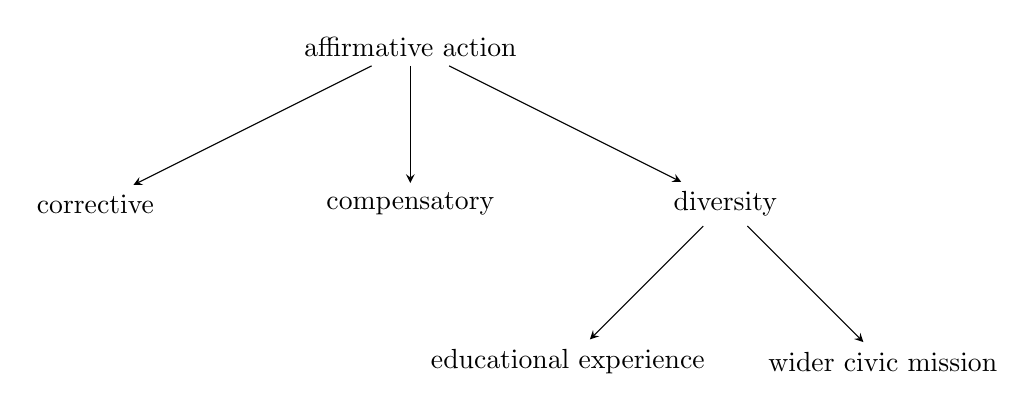
\begin{tikzpicture}[>=stealth]
\node (aa) at (0,0) {affirmative action};
\node (corr) at (-4,-2) {corrective};
\node (comp) at (0,-2) {compensatory};
\node (div) at (4,-2) {diversity};
\node (edu) at (2,-4) {educational experience};
\node (civic) at (6,-4) {wider civic mission};

\draw[->] (aa) -- (corr);
\draw[->] (aa) -- (comp);
\draw[->] (aa) -- (div);
\draw[->] (div) -- (edu);
\draw[->] (div) -- (civic);
\end{tikzpicture}
\end{figure}

The first branch says that students are educated by encountering classmates with different backgrounds and perspectives. The second says that institutions such as law schools train leaders and public officials, so their admissions decisions may properly reflect the civic communities they serve.

\subsection{Question \& Answer}

Is affirmative action compensation for past injustice, and if so is that fair to present applicants?

The compensatory argument has undeniable intuitive force: past injustice can shape present opportunity. But Sandel immediately identifies its hardest objection. If Hopwood did not commit the past wrong, why should she bear the cost of correcting it? Once the question is put in that way, the compensatory argument can succeed only if we are willing to think in terms of collective responsibility or responsibilities that extend across time. Sandel does not resolve that issue here. He isolates it and sets it aside.

\subsection{Question \& Answer}

What exactly are the three distinct arguments for affirmative action, and how does the diversity argument differ from the other two?

The corrective argument remains within the framework of academic merit, though it interprets merit more carefully. The compensatory argument looks backward to historic wrongs. The diversity argument looks neither simply to measurement nor simply to reparation; it looks to the present and future purpose of the institution. That difference in orientation is what makes the diversity argument philosophically deeper and also more vulnerable to a rights-based challenge.

\section{The Diversity Argument and the Rawlsian Rights Objection}

Once the compensatory route has been bracketed, Sandel turns fully to diversity. He presents the University of Texas law school's civic rationale and then invokes the Bakke case, especially Harvard's brief, where race is defended as one ``plus'' factor among many possible contributors to a rich educational environment. Geography, talents, family background, and race all appear in the same list.

The important move here is not the list itself but the principle beneath it. Admission need not be governed by scholarly excellence alone if the institution has a legitimate mission broader than ranking test scores.

At this point the lecture returns to the prior Rawlsian theme. The question is no longer simply whether diversity is good. The question is whether the pursuit of a common good or institutional mission may deny an individual what she claims as her due.

\begin{equation}
\text{common good} \not\Longrightarrow \text{automatic override of individual rights}
\end{equation}

The candidate right is stated in the language of fairness: perhaps an applicant has a right to be judged by achievement, hard work, or at least by factors within her control. But Sandel then presses the opposite reply. Maybe no one morally deserves admission under any supposedly neutral set of criteria, because the criteria themselves are fixed only after the institution defines its purpose.

\begin{equation}
\text{no one morally deserves admission}
\end{equation}

\begin{equation}
\text{institutional mission}
\Longrightarrow
\text{admissions criteria}
\Longrightarrow
\text{legitimate expectations}
\end{equation}

\begin{equation}
\text{desert} \neq \text{entitlement to admission}
\end{equation}

This is the deepest conceptual return of the lecture. We began with Rawls's rejection of desert in distributive justice, and now the admissions debate reproduces the same structure. One may be entitled under a given admissions regime once its mission and rules are fixed, but one does not morally deserve the prior fact that the regime prizes exactly the qualities one happens to possess.

\subsection{Question \& Answer}

Does an applicant have a right to be judged only by achievements and factors within her control?

The lecture's answer is unstable on purpose. The complaint has great intuitive appeal, and Sandel gives it full weight. But the reply is equally strong: many admissions-relevant advantages, including family background, schooling, location, and inherited opportunity, are also beyond our control. Once we see that, the principle ``judge only by what is under individual control'' becomes hard to apply without remainder. That instability is what drives the lecture toward the next stage.

\section{Reset, Institutional Mission, and Historical Counterexamples}

The lecture then crosses a visible seam. A brief flute example appears, and the discussion resumes with a recap: when we ended last time, three arguments had emerged. This reset is not redundant. It prepares a sharper question than before.

Da challenges the idea that a private institution may simply define its mission however it wants. Sandel then puts the challenge into historical form. The University of Texas Law School in the 1950s and Harvard in the 1930s also appealed to institutional mission when defending exclusionary admissions practices. If mission-language could justify those policies, then mission-language by itself cannot settle the present case.

The question becomes whether there is a principled difference between present-day diversity rationales and earlier exclusionary uses of the same style of argument. Hannah proposes one such difference: inclusion rather than exclusion. The discussion then turns to malice. Historic racist and anti-Semitic policies contained an explicit judgment that the excluded groups were less worthy. A present diversity policy, by contrast, may use race instrumentally without expressing such contempt.

Sandel presses the issue one step further. Even if malice is absent, are applicants still being used as instruments of a social purpose? If so, what becomes of the idea that positions, seats, and opportunities should reflect moral desert?

This point is made vivid through the imagined admissions letters. A rejection letter, on this picture, would tell the unsuccessful applicant that society did not need her traits at the moment. An acceptance letter would congratulate the successful applicant only in the weak sense that one congratulates the winner of a lottery. The letters are comic, but they perform serious work: they reveal the moral oddness of detaching admissions entirely from desert while still treating the outcome as worthy of congratulation.

\subsection{Question \& Answer}

Is there a principled difference between today's diversity rationale and earlier exclusionary appeals to institutional mission?

The lecture offers two candidate differences and refuses to let either remain easy. The first is inclusion versus exclusion. The second is absence of malice. Both matter, but neither ends the inquiry. Once we allow mission to structure admissions, we still need an account of why some missions are just and others unjust. That is the point at which a purely Rawlsian or rights-oriented vocabulary starts to feel incomplete.

\section{Aristotle, Flutes, and Teleological Justice}

To challenge the shared anti-desert assumption of modern theories, Sandel turns to Aristotle. Here the lecture acquires a new kind of rigor. The key claim is not merely that people should get what they deserve. It is that what they deserve depends on the nature and purpose of the thing being distributed.

\begin{equation}
\text{justice} = \text{giving each person his or her due}
\end{equation}

\begin{equation}
\text{equal in the relevant respect}
\Longrightarrow
\text{equal things assigned}
\end{equation}

The phrase ``relevant respect'' is the fulcrum. Equal in what respect? Aristotle's answer is: that depends on the good being allocated. Justice is therefore not independent of purpose.

\begin{equation}
\text{telos of the practice}
\Longrightarrow
\text{relevant excellence}
\Longrightarrow
\text{just discrimination / allocation}
\end{equation}

The flute example compresses the whole view into a worked case.

\paragraph{Worked example: the allocation of flutes.}
\begin{enumerate}
\item Ask what is being distributed: flutes.
\item Ask what flutes are for: they are for being played well.
\item Identify the relevant excellence: flute playing.
\item Conclude that the best flutes should go to the best flute players.
\end{enumerate}

In symbols:

\begin{align}
\text{flutes} &\Longrightarrow \text{flute playing},\\
\text{flute playing} &\Longrightarrow \text{relevant excellence},\\
\text{relevant excellence} &\Longrightarrow \text{best flute players get the best flutes.}
\end{align}

This immediately excludes a number of seemingly plausible criteria.

\begin{equation}
\{\text{wealth},\ \text{birth},\ \text{beauty},\ \text{chance}\}
\not\Longrightarrow
\text{just basis for flute allocation}
\end{equation}

Sandel then guards against the most tempting misunderstanding. Aristotle is not giving a utilitarian argument. The reason the best flutes go to the best flute players is not simply that better music will maximize enjoyment. Better music may well follow, but that is a by-product. The point is that the allocation is defined by the telos of the practice.

\subsection{Question \& Answer}

Why should the best flutes go to the best flute players, and why is that answer not utilitarian?

The utilitarian answer would say: because that allocation produces the best consequences. Aristotle's answer is different: because that is what flutes are for. A just distribution is not whatever maximizes aggregate satisfaction; it is whatever fits the purpose of the good and the excellence relevant to it.

That is why Sandel can move from flutes to tennis courts with no change in structure. If the purpose of the court is excellent play, then priority goes to those whose excellence is relevant to that practice, not to the wealthy, the beautiful, or the institutionally influential. The same reasoning, stripped of the ancient background and applied cautiously, invites a final reframing of the admissions debate:

\begin{equation}
\text{affirmative action dispute}
\Longrightarrow
\text{dispute over the telos of university education}
\end{equation}

The lecture closes by widening the frame one last time. Modern thought became suspicious of teleological explanation in nature, but the moral and political question does not disappear so easily. Even if we no longer read nature itself as purposive in Aristotle's way, we still ask what universities are for, what practices are for, and what excellences properly belong to them. That is why the move to Aristotle does not abandon the affirmative-action debate. It explains what kind of debate it has been all along.

\section{Summary}

We began with Rawls's claim that justice is not simply the reward of moral desert, and we watched that claim tested in the setting of admissions. The Hopwood case generated three distinct defenses of affirmative action: correction for unequal preparation, compensation for past wrongs, and diversity in the service of institutional purpose. The hardest version of the debate arose when diversity was defended in the name of the common good and institutional mission, for that argument forced us to ask whether applicants can be denied admission for purposes larger than themselves.

At precisely that point the lecture turned to Aristotle. The resulting lesson is not that affirmative action is settled by a formula. It is that any serious answer will depend on how we understand the purpose of the university and the excellences relevant to it. Justice, in this closing Aristotelian sense, is not blind to purpose. It asks what the practice is for, and only then asks who should rightly receive its goods.